%%%%%%%% ICML 2026 EXAMPLE LATEX SUBMISSION FILE %%%%%%%%%%%%%%%%%

\documentclass{article}

% Recommended, but optional, packages for figures and better typesetting:
\usepackage{microtype}
\usepackage{graphicx}
\usepackage{subcaption}
\usepackage{booktabs} % for professional tables

\usepackage{chngcntr}
\usepackage{apptools}
\AtAppendix{\counterwithin{lemma}{section}}
% hyperref makes hyperlinks in the resulting PDF.
% If your build breaks (sometimes temporarily if a hyperlink spans a page)
% please comment out the following usepackage line and replace
% \usepackage{icml2026} with \usepackage[nohyperref]{icml2026} above.
\usepackage{hyperref}
\usepackage{tikz}
\usepackage{ragged2e}
\usepackage{dsfont}
\usetikzlibrary{positioning, arrows.meta}


% Attempt to make hyperref and algorithmic work together better:
\newcommand{\theHalgorithm}{\arabic{algorithm}}

% Use the following line for the initial blind version submitted for review:
% \usepackage{icml2026}

% For preprint, use
\usepackage[preprint]{icml2026}

% If accepted, instead use the following line for the camera-ready submission:
% \usepackage[accepted]{icml2026}

\usepackage{amsmath}
\usepackage{amssymb}
\usepackage{mathtools}
\usepackage{amsthm}


% if you use cleveref..
\usepackage[capitalize,noabbrev]{cleveref}

%%%%%%%%%%%%%%%%%%%%%%%%%%%%%%%%
% THEOREMS
%%%%%%%%%%%%%%%%%%%%%%%%%%%%%%%%
\theoremstyle{plain}
\newtheorem{theorem}{Theorem}
\newtheorem{proposition}{Proposition}
\newtheorem{lemma}{Lemma}
\newtheorem{corollary}{Corollary}
\theoremstyle{definition}
\newtheorem{definition}{Definition}
\newtheorem{assumption}{Assumption}
\theoremstyle{remark}
\newtheorem{remark}{Remark}

% Todonotes is useful during development; simply uncomment the next line
%    and comment out the line below the next line to turn off comments
%\usepackage[disable,textsize=tiny]{todonotes}
\usepackage[textsize=tiny]{todonotes}

% The \icmltitle you define below is probably too long as a header.
% Therefore, a short form for the running title is supplied here:
\icmltitlerunning{The County-Level Effect of Poverty on Cardiovascular Disease Mortality}

\begin{document}

\twocolumn[
  \icmltitle{The County-Level Effect of Poverty on Cardiovascular Disease Mortality}

  % It is OKAY to include author information, even for blind submissions: the
  % style file will automatically remove it for you unless you've provided
  % the [accepted] option to the icml2026 package.

  % List of affiliations: The first argument should be a (short) identifier you
  % will use later to specify author affiliations Academic affiliations
  % should list Department, University, City, Region, Country Industry
  % affiliations should list Company, City, Region, Country

  % You can specify symbols, otherwise they are numbered in order. Ideally, you
  % should not use this facility. Affiliations will be numbered in order of
  % appearance and this is the preferred way.
  \icmlsetsymbol{equal}{*}

  \begin{icmlauthorlist}
  \icmlauthor{Mathew Chandy}{equal,yyy}
\end{icmlauthorlist}

\icmlaffiliation{yyy}{Department of Statistics and Data Science, University of California, Los Angeles, Los Angeles, CA, USA}
% \icmlaffiliation{comp}{Company Name, Location, Country} % <-- Commented out
% \icmlaffiliation{sch}{School of ZZZ, Institute of WWW, Location, Country} % <-- Commented out

\icmlcorrespondingauthor{Mathew Chandy}{mathewchandy@g.ucla.edu}
  

  % You may provide any keywords that you find helpful for describing your
  % paper; these are used to populate the "keywords" metadata in the PDF but
  % will not be shown in the document
  \icmlkeywords{Machine Learning, ICML}

  \vskip 0.3in
]

% this must go after the closing bracket ] following \twocolumn[ ...

% This command actually creates the footnote in the first column listing the
% affiliations and the copyright notice. The command takes one argument, which
% is text to display at the start of the footnote. The \icmlEqualContribution
% command is standard text for equal contribution. Remove it (just {}) if you
% do not need this facility.

% Use ONE of the following lines. DO NOT remove the command.
% If you have no special notice, KEEP empty braces:
\printAffiliationsAndNotice{}  % no special notice (required even if empty)
% Or, if applicable, use the standard equal contribution text:
% \printAffiliationsAndNotice{\icmlEqualContribution}

\begin{abstract}
Heart disease is the leading cause of death in the United States (reference) and globally. It falls under the broader umbrella of diseases referred to as cardiovascular diseases, which constitutes 1 in 3 deaths in the United States. Therefore, it is of great interest to understand potential causes of cardiovascular disease mortality. These can take the form of more individual variables like level of nutrition and exercise as well as societal factors. The social force of poverty is known to have a link with many negative outcomes, one of these being cardiovascular disease mortality. However, the exact relationship is confounded by many other covariates. We use recent methods developed for continuous treatments to estimate the total causal effect that poverty rate has on the cardiovascular disease mortality rate of a county in the U.S.
\end{abstract}

\section{Introduction}
\label{sec:intro}
My goal for this project is to investigate the causal
relationship between poverty rate and
cardiovascular disease (CVD) mortality rate at the county level. I am using 2016 data from several sources which I merge
by county FIPS code.
The first is the CDC Wonder dataset \citep{cdc_wonder_cmf_data}, which contains
information on age-adjusted CVD mortality rate ($Y$) for counties across the U.S. We use the age-adjusted outcome,
which standardizes to the year-2000 national population, to remove the mechanical effect of county age structure on mortality rates \citep{anderson1998age}.
The second is the American Community Survey, which contains
information on poverty rate ($X$), non-white population ($C$), which serves as a proxy for general racial composition, and \% aged 65 years older ($A$) 
which we retained as a covariate despite the age adjustment because standardization to the year-2000 reference population does not fully eliminate residual age confounding in counties with extreme demographic profiles.
We use the Small Area Health Insurance Estimates (SAHIE)
to obtain uninsurance rate ($M$) and the National Center for Health Statistics (NCHS) to obtain the urbanicity classification ($R$) as defined in 2013.  The urban-rural classification scheme has six ordinal levels:  ...................
% https://www.cdc.gov/nchs/data/data-analysis/2023-File-Documentation-final.pdf. 
%https://www.census.gov/content/dam/Census/library/visualizations/2021/demo/p30-09/F2_Map.pdf
We obtain each county's medicaid expansion status ($G$) as of January 1st, 2016 from KFF.

In Section~\ref{causal_model}, we outline the assumptions of our causal model on which we based our analysis. In 
Section~\ref{data}, we discuss some challenges encountered with this dataset and how we handled missing data. In 
Section~\ref{estimation}, we describe our DML procedure
to identify the total effect and spurious effect of poverty rate on cardiovascular mortality rate. In
Section~\ref{heterogeneity}, we utilize a causal 
forest to conduct an analysis of causal effect heterogeneity. Finally, we discuss our conclusions
in Section~\ref{discussion}.


\section{Causal Model}
\label{causal_model}

Let us write out our causal model, where each county is an observational unit.
Let $\mathbf V = \{X, Y, A, C, M, G, R\}$, and
let $\mathbf  U = \{U_A, U_C,U_G,U_R\}$,
where $A \leftarrow U_A$, $C \leftarrow U_C$,
$G \leftarrow U_G$, and $R \leftarrow U_R$.
Here is a diagram of our assumed causal relationship
model:

\centering
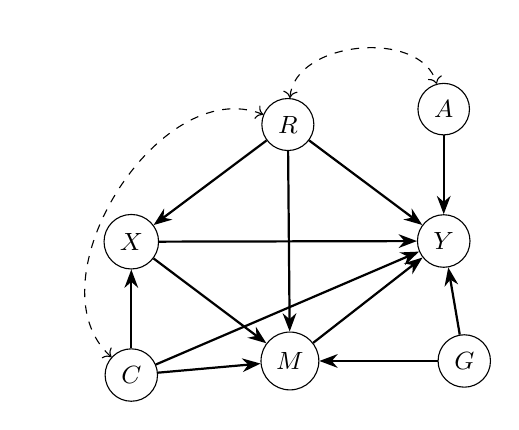
\begin{tikzpicture}[
  node distance = 1cm and 1.5cm,
  every node/.style = {draw, circle, minimum size=0.5cm, font=\small},
  arr/.style = {-{Stealth}, thick}
]


\node (R) {$R$};
\node (X) [below left=of R]  {$X$};
\node (C) [below=of X]       {$C$};
\node (M) [below right=of X] {$M$};
\node (G) [right=of M]       {$G$};
\node (Y) [below right=of R] {$Y$};
\node (A) [above=of Y]       {$A$};

\draw[arr] (X) -- (Y);   % direct effect
\draw[arr] (X) -- (M);   % X -> M
\draw[arr] (M) -- (Y);   % mediated path
\draw[arr] (C) -- (X);   % C -> X
\draw[arr] (C) -- (M);   % C -> M (collider arrow)
\draw[arr] (C) -- (Y);   % C -> Y
\draw[arr] (R) -- (X);   % R -> X
\draw[arr] (R) -- (Y);   % R -> Y
\draw[arr] (R) -- (M);   % R -> M (added: rural uninsurance/access)
\draw[arr] (A) -- (Y);   % age -> Y only
\draw[arr] (G) -- (M);   % Medicaid -> M
\draw[arr] (G) -- (Y);   % Medicaid -> Y (direct, per DiD evidence)
\draw[<->, dashed, bend left=80] (C) to (R);
\draw[<->, dashed, bend left=80] (R) to (A);

\end{tikzpicture}

\justifying






Here is a short review of literature concerning
the causal relationships claimed in our causal diagram.
Poverty directly increases CVD mortality through stress,
malnutrition, and poor housing pathways independent of uninsurance \citep{kim2025mediating}. Poverty also reduces
healthcare access by pricing workers out of employer-sponsored and individual-market coverage, confirmed by the Affordable Care Act (ACA) Medicaid expansion difference-in-differences literature \citep{khatana2019association}, which also supports medicaid expansion as a cause of reduction in both uninsurance and CVD mortality directly and higher uninsurance rates as a cause of increase in CVD mortality. These conclusions are also supported by \citet{miller2021medicaid}, which links Medicaid expansion
to a 9.4\% reduction in annual mortality using individual-level linked survey and death records. Racial composition increases county poverty through structural racism operating via historically accumulated barriers in housing, employment, and lending \citep{bailey2021structural}. Racial composition also independently raises uninsurance rates - disparities persist within income an deducation groups, confirming this edge is not fully mediated by poverty \citep{lee2021convergence}. Lastly, racial composition increases CVD mortality independently of the poverty and uninsurance pathways, with \citet{geronimus2006weathering}
documenting widening racial gaps in biological stress accumulation that are not explained by income. Rural counties typically have higher poverty due to fewer labor markets and potential industrial decline \citep{farrigan2026rural} and higher CVD mortality through
hospital closures and scarcity of cardiologists that may be independent of poverty \citep{loccoh2022rural}.
The level of urbanicity also raises uninsurance rates through lower employer-sponsored coverage availability
and provider network shortages, though the raw uninsurance gap is smaller than the access gap, so this edge is partially but imperfectly captured by the SAHIE uninsurance measure. Finally, how old the population of a county is predicts CVD mortality as a precision variable. We also include a bidirected edge between urbanicity and non-white-population, with racial minorities making up about 22 percent of the American rural population in 2018, and 43 percent of the urban population \citep{castillo2020racial},
and one between urbanicity and county age, supported a trend of ageing in rural counties \citep{monnat2025us, cohen2023aging}.

We also offer a discussion of how we handled missing response data in our causal model. Because of public data documentation \citet{cdc_wonder_cmf_doc},
we do not have to guess the $m$-graph because
the mechanism is deterministic. It is explicitly
stated that mortality rates are suppressed ($R_Y$) if the total
number of deaths $D$ is less than 10:
$$R_Y \leftarrow \mathds{1} \{D < 10\}$$
The number of deaths
$D$ is a product of the population and the crude
mortality rate, which we know can be expressed as a function of age
and adjusted mortality rate. To show these relationships,
the modified DAG is presented below.

\centering
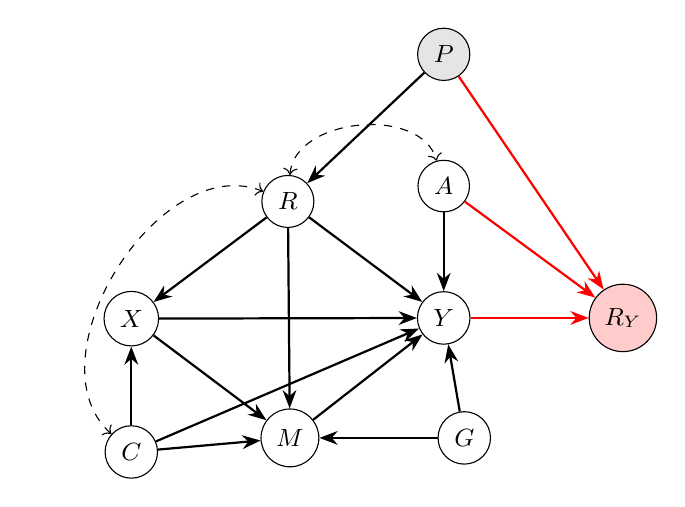
\begin{tikzpicture}[
  node distance = 1cm and 1.5cm,
  every node/.style = {draw, circle, minimum size=0.5cm, font=\small},
  arr/.style = {-{Stealth}, thick}
]

% Existing Nodes
\node (R) {$R$};
\node (X) [below left=of R]  {$X$};
\node (C) [below=of X]       {$C$};
\node (M) [below right=of X] {$M$};
\node (G) [right=of M]       {$G$};
\node (Y) [below right=of R] {$Y$};
\node (A) [above=of Y]       {$A$};

% New Nodes for Missingness
\node (P) [above=of A, fill=gray!20] {$P$}; % Population Size
\node (Ry) [right=of Y, fill=red!20] {$R_Y$}; % Missingness indicator for Y

% Existing Edges
\draw[arr] (X) -- (Y);   
\draw[arr] (X) -- (M);   
\draw[arr] (M) -- (Y);   
\draw[arr] (C) -- (X);   
\draw[arr] (C) -- (M);   
\draw[arr] (C) -- (Y);   
\draw[arr] (R) -- (X);   
\draw[arr] (R) -- (Y);   
\draw[arr] (R) -- (M);   
\draw[arr] (A) -- (Y);   
\draw[arr] (G) -- (M);   
\draw[arr] (G) -- (Y);   
\draw[<->, dashed, bend left=80] (C) to (R);
\draw[<->, dashed, bend left=80] (R) to (A);

% Corrected Population Edges
\draw[arr] (P) -- (R); % Population size determines the NCHS classification

% Edges defining the MNAR missingness mechanism
\draw[arr, draw=red] (P) -- (Ry); % Small populations cause missingness
\draw[arr, draw=red] (Y) -- (Ry); % The true mortality rate determines if deaths < 10
\draw[arr, draw=red] (A) -- (Ry); % Older populations have higher crude rates, preventing missingness

\end{tikzpicture}

\justifying

Here, $R_Y$ is caused by $P$, $A$, and $Y$, which means this is technically an MNAR problem. An edge from
$P$ to $R$ has also been added, because we know $R$ is defined by $P$ from the data documentation of NCHS.
Edges from $P$ to other variables are not justified because any such causal effect would be through $R$'s
causal pathway. In other words, the population of a county is less relevant to many of these societal factors than the population density or urbanicity.

Many variables in this study, including the treatment and the response, are continuous. This necessitates slightly
different notation than in the binary case. Instead of considering two levels $x_0$ and $x_1$ of the treatment poverty rate, we consider some level $x_0$ and 
$x_1 = x_0 + \delta$, where $\delta$ represents some change in the state of $X$.
For instance,
the total variation can be stated as
$$TV_{x_1,x_0}(y)=\mathbb E[Y|X=x_1]-E[Y|X=x_0]$$

I am interested in isolating the direct effect,
indirect effect, and spurious effect. If county poverty increases by $\delta$ percentage points:


\begin{enumerate}
    \item How much does age-adjusted CVD mortality change,
allowing all pathways (healthcare access + stress + structural factors) to operate?
    $$TE_{x_1,x_0}(y) = \mathbb E[Y_{x_1}]-\mathbb E[Y_{x_0}]$$
    \item How much does age-adjusted CVD mortality change,
isolating pathways (stress, housing, nutrition, structural racism channels, etc.) that do not operate through reduced healthcare?
$$NDE_{x_0,x_1}(y) = \mathbb E[Y_{x_1, M_{x_0}}]-\mathbb E[Y_{x_0}]$$
    \item How much does age-adjusted CVD mortality change,
isolating the indirect pathway through uninsurance?
$$NIE_{x_1,x_0}(y) = \mathbb E[Y_{x_1, M_{x_0}}]-\mathbb E[Y_{x_1}]$$
    \item How much of the poverty–mortality association is driven by
racial composition,
rurality,
Medicaid expansion, and 
age structure
rather than poverty itself?
    $$SE_{x_1,x_0}=\mathbb E[Y_{x_1}|x_0] - E[Y_{x_1}|x_1]$$
\end{enumerate}
To make notation a little simpler, we will refer to these effects without their subscripts, $TV_{x_1,x_0}(y)$ with $TV$, for example.


\section{Data}
\label{data}


\section{Estimation of Causal Effects}
\label{estimation}

To identify the total effect of $X$ on $Y$, we can use the backdoor adjustment set to identify $\mathbf Z= \{C,R\}$, which blocks the back-door paths $X\leftarrow C \rightarrow Y$, $X\leftarrow C \rightarrow M\rightarrow Y$, $X \leftarrow R \rightarrow Y$, and 
$X \leftarrow R \rightarrow M\rightarrow Y$. 
While $\{C,R\}$ constitutes the minimal adjustment set
for identifying $TE$, I utilize the expanded set $\mathbf W = \{C,R,A,G\}$, including $A$ and $G$ as precision variables.




% \begin{proof}

% Then we have,
% \[
% \begin{array}{r l l}
% f(Y_{x_1,M_{x_0}}=y) &= \int_m f(Y_{x_1, m}=y,M_{x_0}=m)dm & \text{(CUT)} \\
% &= \int_m f(Y_{x_1, m}=y,M_{x_0}=m)dm & \text{(Chain rule)} \\
% &= Q & \rightarrow\text{E }(1,2)
% \end{array}
% \]
% \end{proof}

Sketch? More flexible than PLM
\begin{enumerate}
    \item Train models with crossfitting (outcome model like XGBoost and density model like ?) on each fold
    \item Debias with influence function on out of fold data
    \item Average
    \item Influence function will have to be shown using strategy 2
    \item Decompose functionals at each data point 
    \item Compute $TV$ with nonparametric regression?
\end{enumerate}

Because of standard causal relationships $TE = NDE - NIE$, and $TV = TE - SE$, 
the minimal procedure requires us to only estimate $TV$, $TE$, and $NDE$. An estimate of the total variation $\widehat {TV}$ can be obtained
with naive nonparametric regression on $X$ alone without adjusting for any other covariates. In our application, we used local linear regression with a Gaussian kernel. The bandwidth was selected by minimizing the cross-validated leave-one-out cross-validation score:
% Assuming a linear relationship, $TV$ would be represented by $\beta_{TV}$ below:
% $$Y=\beta_0 + \beta_{TV} X + \epsilon,$$
% and could be estimated with $\hat \beta_{TV}$ from ordinary least squares. 
An estimate of the total effect $\widehat {TE}$ is slightly more complicated in the continuous setting, and necessitates newer causal tools. We make use of
the framework developed by \citet{kennedy2017non}. First,
let's denote the mean outcome given observed covariates $\mathbf w$ and treatment $x$ with $\mu(\mathbf w, x) = \mathbb E[Y|\mathbf W =\mathbf w, X=x]$, and let's denote
the conditional treatment density given covariates 
with $\pi(x|\mathbf w)= f(x|\mathbf W = \mathbf w)$.

In this setting, we want to obtain a function $\xi(\mathbf V;\pi,\mu)$ of observed data $\mathbf V$ and nuisiance functions
$(\pi, \mu)$
such that
$$\mathbb E[\xi(\mathbf V;\bar\pi,\bar\mu)|X=x]=\mathbb E[Y_x],$$
if at least one of $\bar \pi = \pi$ and $\bar \mu  = \mu$.
After having estimated $\hat \mu$ and $\hat \pi$ with machine learning methods, we can regress $\xi(\mathbf V;\hat\pi,\hat\mu)$ on
$X$ alone as we did to estimate total variation.
From \citet{kennedy2017non}'s Theorem 1,
we estimate the following pseudo-outcome
$$\hat \xi(\mathbf V; \hat \pi, \hat \mu)=\frac{Y-\hat \mu(}{}$$




Then $\widehat {TE}_{x_1,x_0}(y) = \hat \theta + \hat \gamma \hat \alpha$, $\widehat {NDE}_{x_0,x_1}(y) = \hat \theta$, $\widehat {NIE}_{x_1,x_0}(y) = -\hat \gamma \hat \alpha$. 

\section{Causal Effect Heterogeneity}
\label{heterogeneity}
To offer an alternative approach to this problem and
to enable analysis of heterogeneity in causal effect,
we applied a causal forest using the \texttt{grf} package \citep{grf}. When the treatment assignment is binary and unconfounded, this identifies
conditional average treatment effect
$$\tau(\mathbf w) = \mathbb E[Y_{x_1} - Y_{x_0} | \mathbf W = \mathbf w].$$ 
When the treatment is continuous, this identifies 
average partial effect
$$\tau(\mathbf w) = \text{Cov}[Y, X | \mathbf W = \mathbf w] / \text{Var}[X | \mathbf W = \mathbf w],$$ 
which we interpret as a treatment effect given unconfoundedness. Taking the mean of these treatment
effects over the observed data.





\section{Discussion}
\label{discussion}

% Data
% https://wonder.cdc.gov/cmf-icd10.html
% tidycensus

%%%%%%%%%%%%%%%%%%%%%%%%%%%%%%%%%%%%%%%%%%%%%%%%%%%%%%%%%%%%%%%%%%%%%%%%%%%%%%%
%%%%%%%%%%%%%%%%%%%%%%%%%%%%%%%%%%%%%%%%%%%%%%%%%%%%%%%%%%%%%%%%%%%%%%%%%%%%%%%

\bibliography{main}
\bibliographystyle{icml2026}

\end{document}

% This document was modified from the file originally made available by
% Pat Langley and Andrea Danyluk for ICML-2K. This version was created
% by Iain Murray in 2018, and modified by Alexandre Bouchard in
% 2019 and 2021 and by Csaba Szepesvari, Gang Niu and Sivan Sabato in 2022.
% Modified again in 2023 and 2024 by Sivan Sabato and Jonathan Scarlett.
% Previous contributors include Dan Roy, Lise Getoor and Tobias
% Scheffer, which was slightly modified from the 2010 version by
% Thorsten Joachims & Johannes Fuernkranz, slightly modified from the
% 2009 version by Kiri Wagstaff and Sam Roweis's 2008 version, which is
% slightly modified from Prasad Tadepalli's 2007 version which is a
% lightly changed version of the previous year's version by Andrew
% Moore, which was in turn edited from those of Kristian Kersting and
% Codrina Lauth. Alex Smola contributed to the algorithmic style files.
